%%%%%%%%%%%%%%%%%%%%%%%%%%%%%%%%%%%%%%%%%%%%%%%%%%%%%%%%%%%%%%%
%
% Welcome to Overleaf --- just edit your LaTeX on the left,
% and we'll compile it for you on the right. If you open the
% 'Share' menu, you can invite other users to edit at the same
% time. See www.overleaf.com/learn for more info. Enjoy!
%
%%%%%%%%%%%%%%%%%%%%%%%%%%%%%%%%%%%%%%%%%%%%%%%%%%%%%%%%%%%%%%%
\documentclass{article}
% \usepackage[utf8]{inputenc} is no longer required (since 2018)

% Set the font (output) encoding
\usepackage[LGR]{fontenc}
\usepackage{multirow}
\usepackage{enumitem}
\usepackage{moreenum}
\usepackage{pgfplots}

\pgfkeys{/pgfplots/Axis Style/.style={
    width=8.5cm, height=8.5cm,
    samples=100,
    ymin=-1, ymax=1,
    xmin=-4, xmax=4,
    domain=-pi:pi
}}


% Greek-specific commands
\usepackage[greek]{babel}
 \title{Εργασία \textlatin {\LaTeX}} % Put your own title here

% * Setting the author or authors of the document
 \author{Όνοματεπώνυμο: Δημήτριος Αθανασιάδης  \\  ΑΕΜ: 3724}       % Put your own Name and AEM here

% * Setting the date of the document
  \date{10 Νοεμβρίου 2021}   
\begin{document}
\maketitle

\section{Πρώτη Άσκηση}
\begin{center}
\tinyΑ\scriptsizeΒ\footnotesizeΓ\smallΔ\normalsizeΕ\largeΖ\LARGEΗ\hugeΘ\HugeΙ\hugeκ\LARGEλ\largeμ\normalsizeν\smallξ\footnotesizeο\scriptsizeρ\tinyσ
\end{center}

\section{Δεύτερη άσκηση}
\begin{center}
\textlatin{\textit{Normal Italics \textbf{Bold}}\\ E\emph{mphasized}  \textit{\underline{Underlined}}}
\end{center}

\section{Τρίτη άσκηση}
\begin{equation*}
a^2 + b^2 = c^2 \\
\end{equation*}
\begin{equation*}
e^{i\pi} = -1 \\
\end{equation*}
\begin{equation*}
\pi = \frac{c}{d} \\
\end{equation*}
\begin{equation*}
\frac{d}{dx} \int_{a}^{x} f(s)ds=f(x) \\
\end{equation*}
\begin{equation*}
f(x) = \sum_{i=0}^{\infty} \frac{f^{(i)}(0)}{i!}x^i \\ 
\end{equation*}
\begin{equation*}
\textbf{\textlatin{Ax = b}} \\
\end{equation*}
\begin{equation*}
||x+y|| \leq ||x|| + ||y||
\end{equation*} \\
\begin{equation}
    \textbf{I}=\begin{pmatrix}
    1&0&0&0 \\
    0&1&0&0 \\
    0&0&1&0 \\
    0&0&0&1
    \end{pmatrix}
\end{equation} \\
\begin{equation}
    \textbf{I}=\begin{bmatrix}
    1&0&0&0 \\
    0&1&0&0 \\
    0&0&1&0 \\
    0&0&0&1
    \end{bmatrix}
\end{equation} \\
\begin{equation}
    \textbf{I}=\begin{Bmatrix}
    1&0&0&0 \\
    0&1&0&0 \\
    0&0&1&0 \\
    0&0&0&1
    \end{Bmatrix},\;\;\;
    \textbf{I}=\begin{vmatrix}
    1&0&0&0 \\
    0&1&0&0 \\
    0&0&1&0 \\
    0&0&0&1
    \end{vmatrix},\;\;\;
    \textbf{I}=\begin{Vmatrix}
    1&0&0&0 \\
    0&1&0&0 \\
    0&0&1&0 \\
    0&0&0&1
    \end{Vmatrix}
\end{equation}
\bigskip
\section{Τέταρτη άσκηση} \bigskip
\begin{center}
\begin{tabular}{ l c r }
  Τεφάς & 2 & 3 \\
  Πήτας & 5 & 6 \\
  Λάσκαρης & 8 & 9 \\
\end{tabular} \\\bigskip\medskip
\begin{tabular}{| l | c | r |}
  Κοτρόπουλος & 6 & 3 \\
  Πήτας & 5 & 6 \\
  Νικολαίδης & 8 & 9 \\
\end{tabular}  \\\bigskip\medskip
\begin{tabular}{ | c | c | c |}
    \hline
    1 & 2 & 3 \\ \hline
    4 & 5 & 6 \\ \hline
    7 & 8 & 9 \\
    \hline
\end{tabular}  \\\bigskip\medskip
\begin{tabular}{ | c | c | c |}
    \hline
    1 & 2 & 3 \\ \hline
    4 & 5 & 6 \\ \hline
    7 & 8 & 9 \\
    \hline
\end{tabular}  \\\bigskip\medskip
\begin{tabular}{|l|c|l|}
  \hline
  \multicolumn{3}{|c|}{Μέλη ΔΕΠ Πληροφορικής} \\ \hline
  Λέκτορες & \textlatin{VD} & Δραζιώτης Κωνσταντίνος \\ \hline
  \multirow{2}{*}{Επίκουροι} & \textlatin{LN} & Λάσκαρης Νικόλαος \\
  & \textlatin{TG} & Τσουμάκας Γρηγόριος \\ \hline
  \multirow{3}{*}{Αναπληρωτές} & \textlatin{TA} & Τέφας Αναστάσιος \\
  & \textlatin{PN} & Πλέρος Νίκος \\ & \textlatin{PA} & Παπαδόπουλος Απόστολος \\ \hline
  \multirow{3}{*}{Καθηγητές} & \textlatin{KC} & Κοτρόπουλος Κωνσταντίνος \\
  & \textlatin{PI} & Πήτας Ιωάννης \\ & \textlatin{VI} & Βλαχάβας Ιωάννης \\ \hline
\end{tabular}
\end{center}
\newpage

\section{Πέμπτη άσκηση}
\begin{center} \bigskip
\begin{itemize}
\item \textit{Τέφας}
\item \textit{Μπουζάς}
\item \textit{Μπρούζα}
\item \textit{Λάσκαρης}
\item \textit{Κοτρόπουλος}
\item \textit{Πήτας}
\item \textit{Νικολαΐδης}
\end{itemize}
\begin{enumerate}
\item \textit{Τέφας}
\item \textit{Μπουζάς}
\item \textit{Μπρούζα}
\item \textit{Λάσκαρης}
\item \textit{Κοτρόπουλος}
\item \textit{Πήτας}
\item \textit{Νικολαΐδης}
\end{enumerate}
\begin{enumerate}[label=\textbf{(\greek*)}]
\item \textit{Τέφας}
\item \textit{Μπουζάς}
\item \textit{Μπρούζα}
\item \textit{Λάσκαρης}
\item \textit{Κοτρόπουλος}
\item \textit{Πήτας}
\item \textit{Νικολαΐδης}
\end{enumerate}
\end{center}

\section{Έκτη άσκηση} \bigskip
\begin{center}
\pgfplotsset{every tick label/.append style={font=\small}}
\pgfplotsset{label style={font=\tiny},}
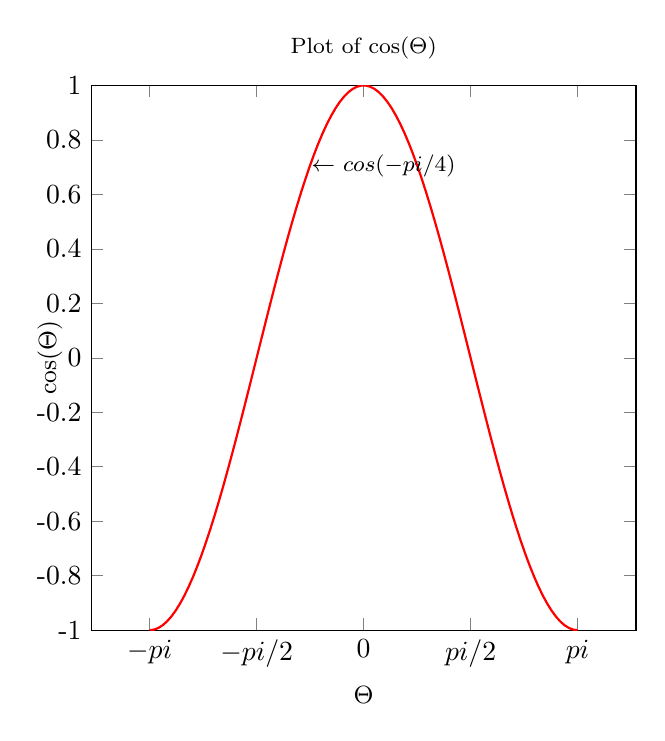
\begin{tikzpicture}
\begin{axis}[
    title={\footnotesize\textlatin{Plot of cos($\Theta$)}},
    Axis Style,
    nodes near coords align=right,
    xlabel={$\Theta$},
    x label style={anchor=north,font=\small},
    ylabel=$\cos(\Theta$),
    y label style={anchor=north,font=\small},
    xtick={
        -3.14159, -1.5708, 0,
        1.5708, 3.14159
    },
    xticklabels={
         $-pi$, $-pi/2$, $0$, $pi/2$, $pi$
    },
    ytick={
        -1, -0.8, -0.6, -0.4, -0.2, 0, 0.2, 0.4, 0.6, 0.8, 1
    },
    yticklabels={
        -1, -0.8, -0.6, -0.4, -0.2, 0, 0.2, 0.4, 0.6, 0.8, 1
    }
]
\addplot [mark=none, thick, red] {cos(deg(x))};
\addplot[mark=none] coordinates {(-3.14159/4,0.7071)} node[label=0:{\footnotesize$\leftarrow$ $cos(-pi/4)$}] at (axis cs:-1.05,0.705) {} ;
\end{axis}
\end{tikzpicture}
\end{center}


\begin{center}
\pgfplotsset{every tick label/.append style={font=\small}}
\pgfplotsset{label style={font=\tiny},}
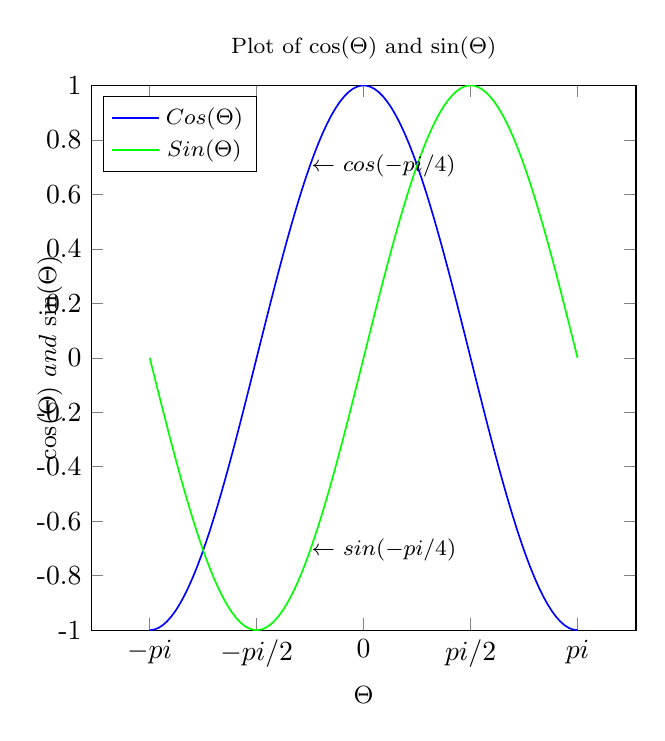
\begin{tikzpicture}
\begin{axis}[
    title={\footnotesize\textlatin{Plot of cos($\Theta$) and sin($\Theta$)}},
    Axis Style,
    nodes near coords align=right,
    xlabel={$\Theta$},
    x label style={anchor=north,font=\small},
    ylabel={$\cos(\Theta)$ $and$ $\sin(\Theta)$},
    y label style={anchor=north,font=\small},
    legend style={at={(0.305,0.98)},font=\footnotesize},
    xtick={
        -3.14159, -1.5708, 0,
        1.5708, 3.14159
    },
    xticklabels={
         $-pi$, $-pi/2$, $0$, $pi/2$, $pi$
    },
    ytick={
        -1, -0.8, -0.6, -0.4, -0.2, 0, 0.2, 0.4, 0.6, 0.8, 1
    },
    yticklabels={
        -1, -0.8, -0.6, -0.4, -0.2, 0, 0.2, 0.4, 0.6, 0.8, 1
    }
]
\addplot [mark=none, semithick, blue] {cos(deg(x))};
\addplot [mark=none, semithick, green] {sin(deg(x))};
\addplot[mark=none] coordinates {(-3.14159/4,0.7071)} node[label=0:{\footnotesize$\leftarrow$ $cos(-pi/4)$}] at (axis cs:-1.05,0.705) {} ;
\addplot[mark=none] coordinates {(-3.14159/4,-0.7071)} node[label=0:{\footnotesize$\leftarrow$ $sin(-pi/4)$}] at (axis cs:-1.05,-0.705) {} ;
\legend{$Cos(\Theta)$,$Sin(\Theta)$}
\end{axis}
\end{tikzpicture}
\end{center}

\end{document}